
\section{Introduction}


\begin{figure}[ht!]
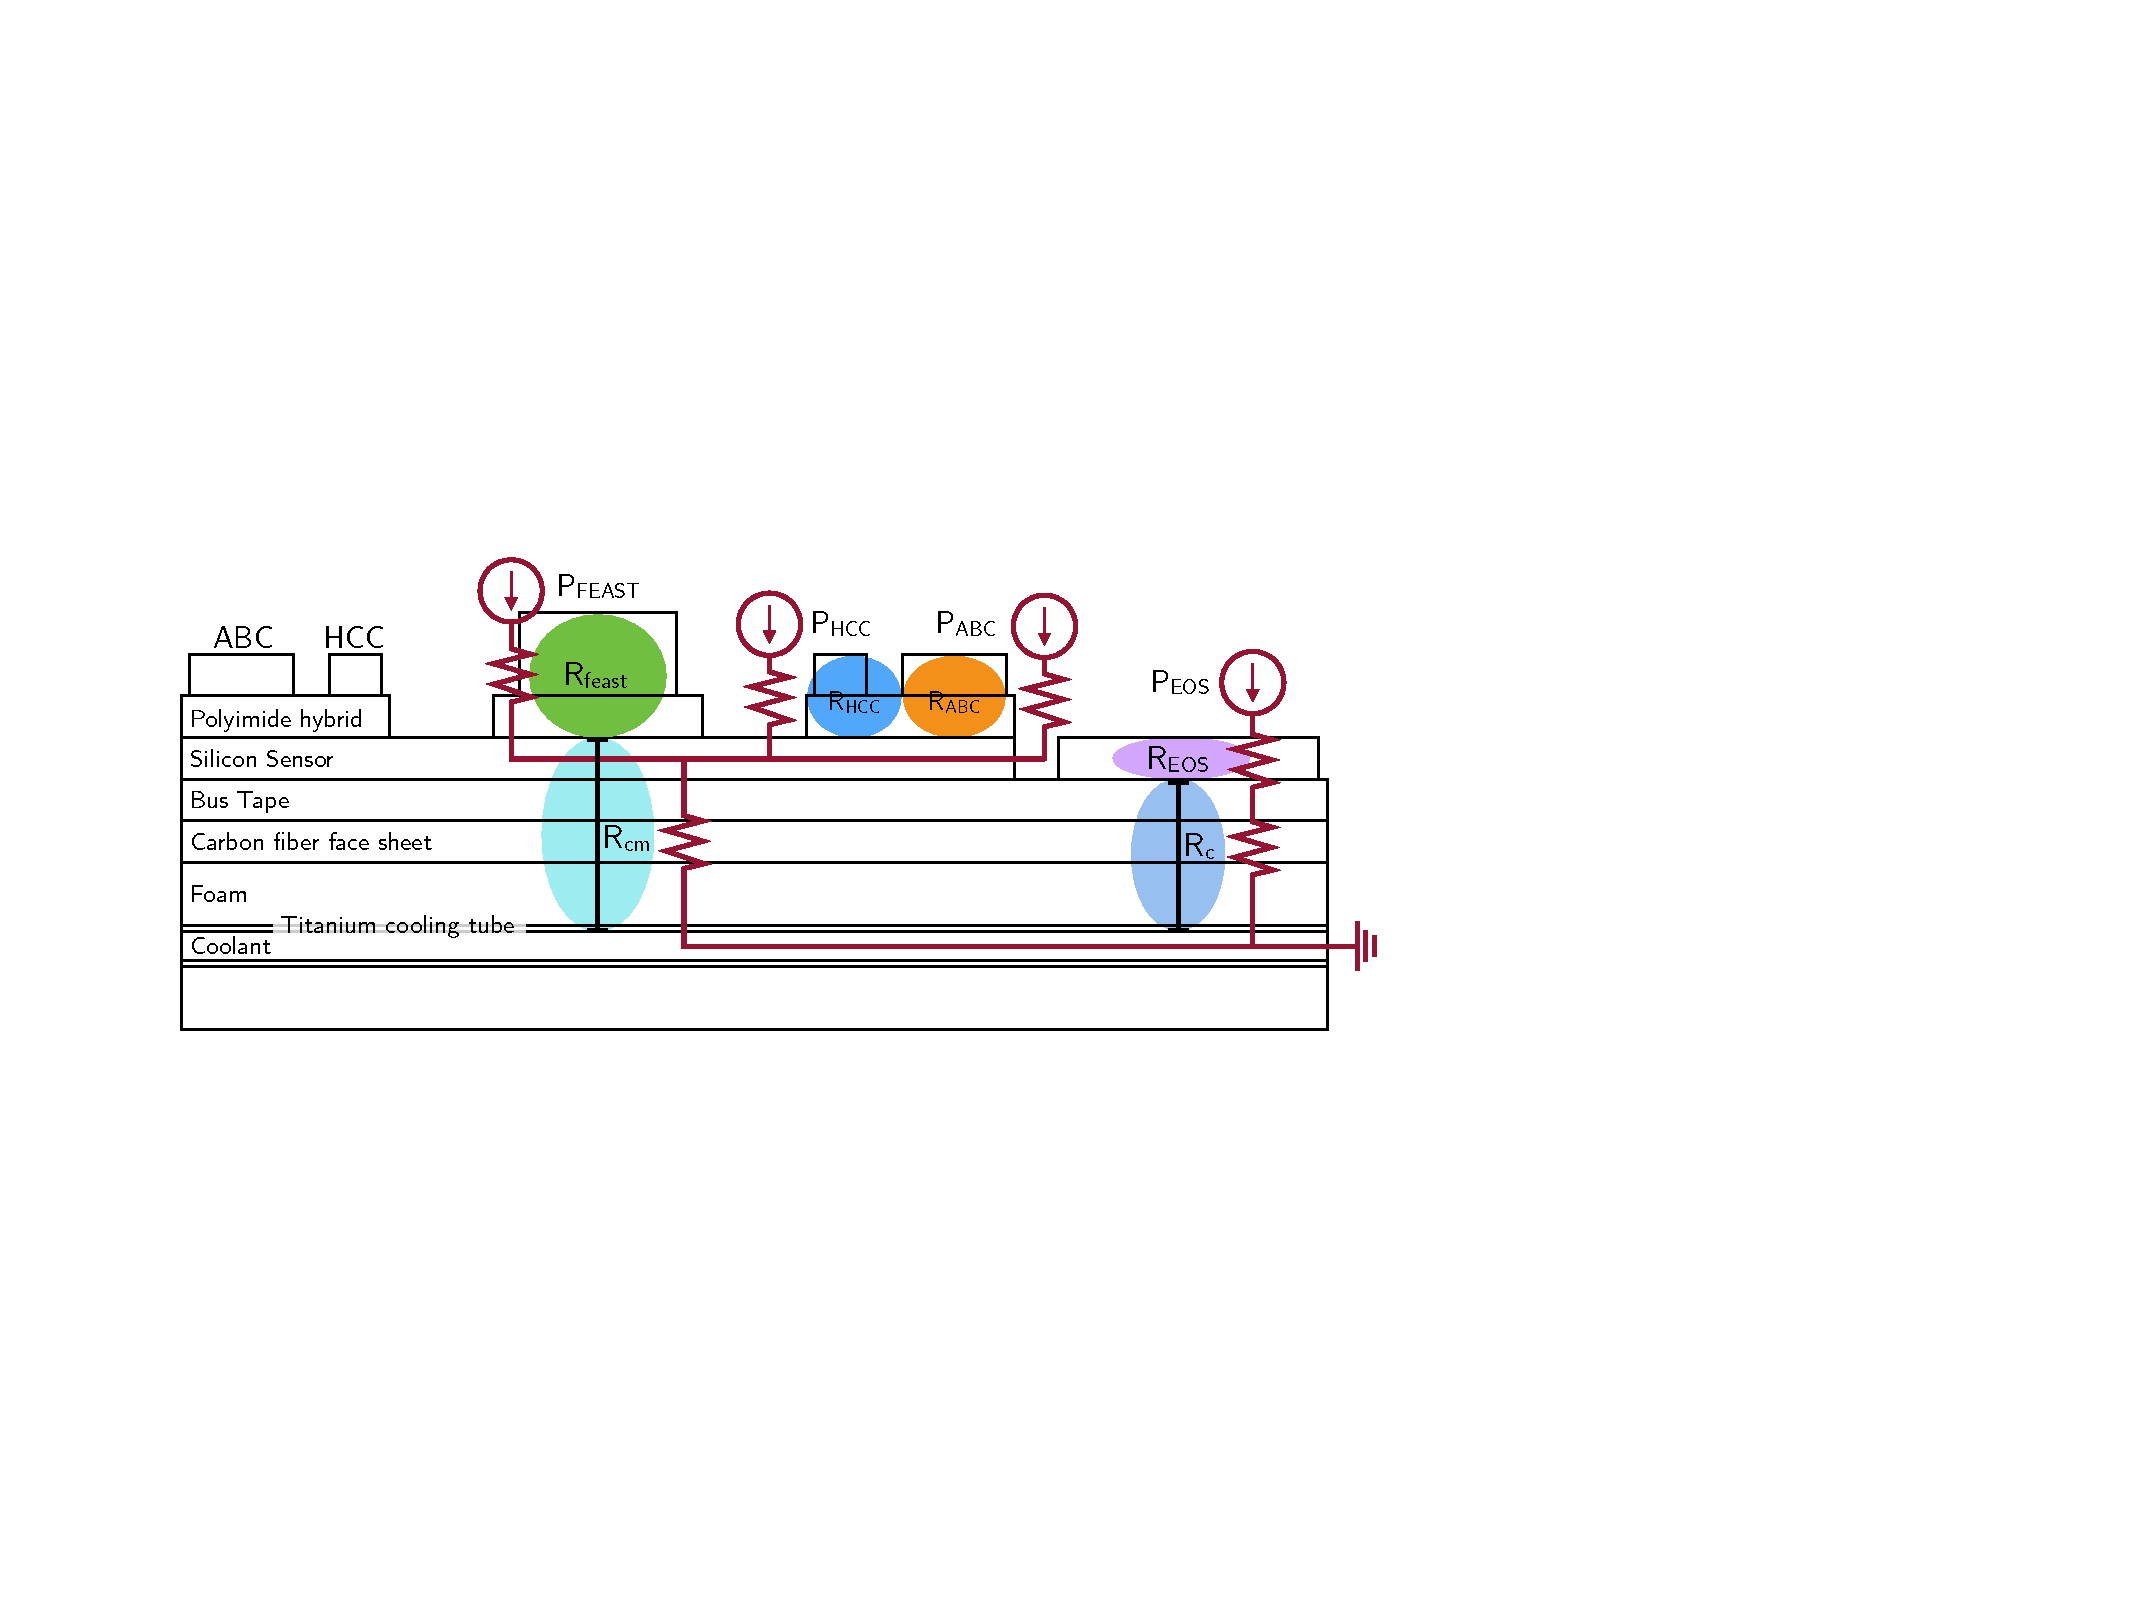
\includegraphics[width=.99\textwidth]{figures/thermoelectric_model.pdf}
\caption{
The thermo-electric model, its analogy with electrical circuits, and definitions of terms.
}
\label{thermoelectric_model}
\end{figure}

Note that e.g. all ABCs are treated as a single node in this description, meaning the ABC power refers
to the total power in all ABCs, and the thermal resistance is an effective thermal resistance for all
ABCs (the same applies to the FEAST and HCC).

Note that the effect of the AMAC as a power source affecting the module temperature is neglected in
the following; however, the AMAC represents roughly 1\% of the total module power, so the impact on
the temperatures of the module is negligible. (The AMAC power itself is counted as part of the total
module power.)

The pathway shared by the EOS and the other components is called $R_{C}$, and is also fit using the
data by measuring the temperature. The two are related according to $R_{CM} = R_C + R_M$.

\subsection{Similarities and differences between the Barrel and Endcap models}

Unless otherwise stated, the Barrel and Endcap models are identical. This includes:
\begin{itemize}
  \item The parameterization used to model the TID bump
  \item The parameterization used to model the FEAST efficiency as a function of temperature 
    and current
  \item The procedure used to extract thermal impedances from thermal FEA simulations
  \item The thermal model itself, which calculates the temperature and power of each component in 
    one-month steps. The endcap model was copied from and validated against an early version
    of the barrel model.
\end{itemize}

Key differences include:
\begin{itemize}
  \item The values of the thermal impedances of each component (due to geometric differences between
    barrel and endcap modules)
  \item The uncertainty (safety factor) of the thermal impedances in the endcap is set to 20\% (as
    opposed to 10\% in the endcap), because the modules have more irregular shapes and the layout of
    powered components is less regular, causing less linear thermal behavior.
\end{itemize}
